\documentclass[main.tex]{subfiles}
\begin{document}

\href{https://www2.seas.gwu.edu/~simhaweb/quantum/modules/module5/module5.html}{Module 5: Multiple Qubits - Measurement and Modification}\\
\href{https://www2.seas.gwu.edu/~simhaweb/quantum/modules/module5/problems5.html}{Module-5 Solved Problems}

\begin{enumerate}

\item[] \textbf{In-Class Exercise 1:} Consider the single-qubit projectors $P_{+}=|+\rangle\langle+|$ and $P_{-}=|-\rangle\langle-|$.
    \begin{enumerate}
        \item[1.] \textbf{Q.} Show that $\left(P_{+} \otimes I\right)|00\rangle=\frac{1}{\sqrt{2}}|+, 0\rangle$ and $\left(P_{+} \otimes I\right)|11\rangle=\frac{1}{\sqrt{2}}|+, 1\rangle$ \textbf{A.}
        \begin{align*}
            \left(P_{+} \otimes I\right) |00\rangle & = |+\rangle \langle+|0\rangle \otimes I |0\rangle\\
                                                    & = \frac{1}{\sqrt{2}} |+\rangle \otimes |0\rangle\\
                                                    & = \frac{1}{\sqrt{2}} |+,0\rangle\\
            \left(P_{+} \otimes I\right)|11\rangle  & = |+\rangle \langle+|1\rangle \otimes I|1\rangle\\
                                                    & = \frac{1}{\sqrt{2}} |+\rangle \otimes |1\rangle\\
                                                    & = \frac{1}{\sqrt{2}} |+,1\rangle
        \end{align*}
        \item[2.] Show that $\frac{1}{\sqrt{2}}|+, 0\rangle+\frac{1}{\sqrt{2}}|+, 1\rangle=|+,+\rangle$
        \begin{align*}
            \frac{1}{\sqrt{2}}|+, 0\rangle
            + \frac{1}{\sqrt{2}}|+, 1\rangle    & = |+\rangle \otimes \left(\frac{1}{\sqrt{2}}| 0\rangle
                                                + \frac{1}{\sqrt{2}}| 1\rangle \right) \\
                                                & = |+,+\rangle 
        \end{align*}
        \item[3.] Expand $\left(P_{+} \otimes I\right)$ into a matrix and use that to show $\left(P_{+} \otimes I\right)|\psi\rangle=|+,+\rangle$ (normalized) where $|\psi\rangle=\frac{1}{\sqrt{2}}(|00\rangle+|11\rangle)$
        \begin{align*}
            \left(P_{+}\otimes I\right) & = \left[\begin{array}{ll} \frac{1}{2} & \frac{1}{2} \\
                                        \frac{1}{2} & \frac{1}{2}\end{array}\right] 
                                        \otimes \left[\begin{array}{ll} 1 & 0 \\
                                        0 & 1\end{array}\right]\\
                                        & = \frac{1}{2}\left[\begin{array}{llll}1&1&0&0\\
                                        1&1&0&0\\
                                        0&0&1&1\\
                                        0&0&1&1\\\end{array}\right]\\
            \left(P_{+}\otimes I\right)
            |\psi\rangle                & = \frac{1}{2\sqrt{2}}\left[\begin{array}{llll}1&1&0&0\\
                                        1&1&0&0\\
                                        0&0&1&1\\
                                        0&0&1&1\\\end{array}\right]
                                        \left[\begin{array}{l}1\\1\\1\\1\end{array}\right]\\
                                        & = \frac{1}{\sqrt{2}} \left[\begin{array}{l}1\\1\\1\\1\end{array}\right]\\
                                        & = \sqrt{2} |+,+\rangle \tag{normalized}
        \end{align*}
    \end{enumerate}

\item[] \textbf{In-Class Exercise 2:} \textbf{Q.} Apply the projectors $\left(P_{+} \otimes I\right)$ and $\left(P_{-} \otimes I\right)$ to $|\psi\rangle=\frac{1}{2}(|00\rangle+|01\rangle+|10\rangle+|11\rangle$ using the Dirac-notation approach above, and then confirm your results by expanding into matrices. \textbf{A.}
    \begin{align*}
        \left(P_{+} \otimes I\right)|\psi\rangle    & = \frac{1}{2}(|+\rangle\langle+|\otimes I)
                                                    (|00\rangle+|01\rangle+|10\rangle+|11\rangle)\\
                                                    & = \frac{1}{2}(|+\rangle\langle+|\otimes I)
                                                    (|0\rangle\otimes|0\rangle + |0\rangle\otimes|1\rangle +
                                                    |1\rangle\otimes|0\rangle + |1\rangle\otimes|1\rangle)\\
                                                    & = \frac{1}{2}(|+\rangle\langle+|0\rangle\otimes I|0\rangle + |+\rangle\langle+|0\rangle\otimes I|1\rangle +
                                                    |+\rangle\langle+|1\rangle\otimes I|0\rangle + 
                                                    |+\rangle\langle+|1\rangle\otimes I|1\rangle)\\ 
                                                    & = \frac{1}{2\sqrt{2}}(|+,0\rangle + |+,1\rangle + |+,0\rangle + |+,1\rangle)\\
                                                    & = \frac{1}{\sqrt{2}}|+\rangle\frac{1}{\sqrt{2}}(|0\rangle+|1\rangle)\\
                                                    & = \frac{1}{\sqrt{2}}|+,+\rangle\\
                                                    & = |+,+\rangle \tag{normalized}\\ 
        \left(P_{+} \otimes I\right)|\psi\rangle    & = \frac{1}{4}\left[\begin{array}{llll}1&0&1&0\\0&1&0&1\\
                                                    1&0&1&0\\0&1&0&1\end{array}\right]
                                                    \left[\begin{array}{l}1\\1\\1\\1\end{array}\right]\\
                                                    & = \frac{1}{2} \left[\begin{array}{l}1\\1\\1\\1\end{array}\right]\\
        \left(P_{-} \otimes I\right)|\psi\rangle    & = \frac{1}{2}(|-\rangle\langle-|\otimes I)
                                                    (|00\rangle+|01\rangle+|10\rangle+|11\rangle)\\
                                                    & = \frac{1}{2}(|-\rangle\langle-|\otimes I)
                                                    (|0\rangle\otimes|0\rangle + |0\rangle\otimes|1\rangle +
                                                    |1\rangle\otimes|0\rangle + |1\rangle\otimes|1\rangle)\\
                                                    & = \frac{1}{2}(|-\rangle\langle-|0\rangle\otimes I|0\rangle + |-\rangle\langle-|0\rangle\otimes I|1\rangle +
                                                    |-\rangle\langle-|1\rangle\otimes I|0\rangle + 
                                                    |-\rangle\langle-|1\rangle\otimes I|1\rangle)\\
                                                    & = \frac{1}{2\sqrt{2}}(|-,0\rangle + |-,1\rangle - |-,0\rangle - |-,1\rangle)\\
                                                    & = 0\\
        \left(P_{-} \otimes I\right)|\psi\rangle    & = \frac{1}{4}\left[\begin{array}{llll}1&0&-1&0\\0&1&0&-1\\
                                                    -1&0&1&0\\0&-1&0&1\end{array}\right]
                                                    \left[\begin{array}{l}1\\1\\1\\1\end{array}\right]\\
                                                    & = \left[\begin{array}{l}0\\0\\0\\0\end{array}\right]
    \end{align*}

\item[] \textbf{In-Class Exercise 3:} Fill in the missing step of normalization in the above example. Then, apply the same projectors to the vector $|\psi\rangle=|+,+,+\rangle$ and list the outcomes and probabilities.
    \begin{align*}
        P_{V_{1}}                           & = |000\rangle\langle 000|
                                            +|010\rangle\langle 010|
                                            +|101\rangle\langle 101|
                                            +|111\rangle\langle 111| \\
        P_{V_{2}}                           & = |001\rangle\langle 001|
                                            +|011\rangle\langle 011|
                                            +|100\rangle\langle 100|
                                            +|110\rangle\langle 110| \\
        |\psi\rangle                        & = \frac{1}{\sqrt{3}}(|000\rangle+|001\rangle+|010\rangle)\\
        P_{V_{1}}|\psi\rangle               & = \frac{1}{\sqrt{3}}(|000\rangle+|010\rangle) \\
        \frac{1}{|P_{V_{1}}|\psi\rangle|}
        P_{V_{1}}|\psi\rangle               & = \frac{\sqrt{3}}{\sqrt{2}}\frac{1}{\sqrt{3}}(|000\rangle+|010\rangle)\\
        \frac{1}{\sqrt{2}}
        (|000\rangle+|010\rangle)           & \text{ with probability } \frac{2}{3}\\
        P_{V_{2}}|\psi\rangle               & = \frac{1}{\sqrt{3}}|001\rangle\\
        \frac{1}{|P_{V_{2}}|\psi\rangle|}
        P_{V_{2}}|\psi\rangle               & = \frac{\sqrt{3}}{1}\frac{1}{\sqrt{3}}|001\rangle\\
        |001\rangle                         & \text{ with probability } \frac{1}{3}\\
        P_{V_{1}}|\psi\rangle               & = P_{V_{1}}\mid+,+,+\rangle\\
                                            & = \frac{1}{2\sqrt{2}}\left(|000\rangle+|010\rangle
                                            +|101\rangle+|111\rangle\right)\\
        \frac{1}{|P_{V_{1}}|\psi\rangle|}
        P_{V_{1}}|\psi\rangle               & = \frac{\sqrt{2}}{1}\frac{1}{2\sqrt{2}}\left(|000\rangle+|010\rangle
                                            +|101\rangle+|111\rangle\right)\\
        \frac{1}{2}(|000\rangle+|010\rangle
        +|101\rangle+|111\rangle)           & \text{ with probability } \frac{1}{2}\\
        P_{V_{2}}|\psi\rangle               & = P_{V_{2}}\mid+,+,+\rangle\\
                                            & = \frac{1}{2\sqrt{2}}\left(|001\rangle+|011\rangle
                                            +|100\rangle+|110\rangle\right)\\
        \frac{1}{|P_{V_{2}}|\psi\rangle|}
        P_{V_{2}}|\psi\rangle               & = \frac{\sqrt{2}}{1}\frac{1}{2\sqrt{2}}\left(|001\rangle+|011\rangle
                                            +|100\rangle+|110\rangle\right)\\
        \frac{1}{2}(|001\rangle+|011\rangle
        +|100\rangle+|110\rangle)     & \text{ with probability } \frac{1}{2}
    \end{align*}

\item[] \textbf{In-Class Exercise 4:} \textbf{Q.} There was one step missing in the sequence of projections above: what happened to the terms $\sqrt{|\alpha|^{2}+|\beta|^{2}}$ and $\sqrt{|\gamma|^{2}+|\delta|^{2}}$ ? Hint: write down the probabilities  $|P_{0}| \psi\rangle|^{2}$ and $|P_{2}| \psi_{0}\rangle|^{2}$, and then ask: what product of probabilities leads us to observing $|00\rangle$ as the outcome? \textbf{A.} The terms multiply to 1 when calculating the product of the two probabilities.
    \begin{align*}
        |P_{0}| \psi\rangle|^{2}        & = |\alpha|^{2}+|\beta|^{2}\\
        |P_{2}| \psi_{0}\rangle|^{2}    & = \frac{\alpha^2}{|\alpha|^{2}+|\beta|^{2}}\\
        |P_{0}| \psi\rangle|^{2} 
        \times |P_{2}| 
        \psi_{0}\rangle|^{2}            & = |\alpha|^2
    \end{align*}

\item[] \textbf{In-Class Exercise 5:}
\begin{enumerate}
    \item[1.] \textbf{Q.} Show that $X^{2}=I$ both with matrix and Dirac forms. \textbf{A.}
    \begin{align*}
        X^2 & = \left[\begin{array}{ll}0&1\\1&0\end{array}\right]
            \left[\begin{array}{ll}0&1\\1&0\end{array}\right]
            = (|0\rangle\langle1| + |1\rangle\langle0|)(|0\rangle\langle1| + |1\rangle\langle0|)\\
            & = \left[\begin{array}{ll}1&0\\0&1\end{array}\right] 
            = |0\rangle\langle0| + |1\rangle\langle1|\\
            & = I
    \end{align*}
    \item[2.] \textbf{Q.} Write out the matrix and Dirac forms of $X \otimes X$. \textbf{A.}
    \begin{align*}
        X \otimes X & = \left[\begin{array}{ll} 0 \left[\begin{array}{ll}0&1\\1&0\end{array}\right] & 
                    1 \left[\begin{array}{ll}0&1\\1&0\end{array}\right] \\
                    1 \left[\begin{array}{ll}0&1\\1&0\end{array}\right] &
                    0 \left[\begin{array}{ll}0&1\\1&0\end{array}\right] \end{array} \right]
                    = (|0\rangle\langle1| + |1\rangle\langle0|) \otimes (|0\rangle\langle1| + |1\rangle\langle0|)\\
                    & = \left[\begin{array}{llll}0&0&0&1\\0&0&1&0\\0&1&0&0\\1&0&0&0\end{array}\right]
                    = |00\rangle\langle11| + |01\rangle\langl10| + |10\rangle\langle01| + |11\rangle\langle00|
    \end{align*}
\end{enumerate}

\item[] \textbf{In-Class Exercise 6:} \textbf{Q.} Confirm the above result with the matrix form of $(I \otimes X)|\psi\rangle$. \textbf{A.}

    \begin{align*}
        (I \otimes X)|\psi\rangle   & = \left[\begin{array}{llll}0&1&0&0\\1&0&0&0\\0&0&0&1\\0&0&1&0\end{array}\right]
                                    \left[\begin{array}{l}\alpha\\\beta\\\gamma\\\delta\end{array}\right]\\
                                    & = \left[\begin{array}{l}\beta\\\alpha\\\delta\\\gamma\end{array}\right]
    \end{align*}

\item[] \textbf{In-Class Exercise 7:} Write down the matrices for $H^{\otimes 2}$ and  $H^{\otimes 3}$ in the above form (pulling out $\frac{1}{\sqrt{2^{n}}}$). This is admittedly a bit tedious but will be useful when we analyze the structure of this matrix for algorithmic insight.

    \begin{align*}
        H^{\otimes 2}   & = \frac{1}{\sqrt{2^2}} \left[\begin{array}{llll}1&1&1&1\\1&-1&1&-1\\
                        1&1&-1&-1\\1&-1&-1&1\end{array}\right]\\
        H^{\otimes 3}   & = \frac{1}{\sqrt{2^3}} \left[\begin{array}{llllllll}1&1&1&1&1&1&1&1\\
                        1&-1&1&-1&1&-1&1&-1\\
                        1&1&-1&-1&1&1&-1&-1\\
                        1&-1&-1&1&1&-1&-1&1\\
                        1&1&1&1&-1&-1&-1&-1\\
                        1&-1&1&-1&-1&1&-1&1\\
                        1&1&-1&-1&-1&-1&1&1\\
                        1&-1&-1&1&-1&1&1&-1\end{array}\right]     
    \end{align*}

\item[] \textbf{In-Class Exercise 8:}
    \begin{enumerate}
        \item[1.] \textbf{Q.} Use the Dirac form to apply $C_{\text{NOT}}$ to $|\psi\rangle=(\alpha|0\rangle+\beta|1\rangle) \otimes |0\rangle$ and $\left|\psi^{\prime}\right\rangle=(\alpha|0\rangle+\beta|1\rangle) \otimes |1\rangle$. \textbf{A.} 
        \begin{align*}
            C_{\text{NOT}}|\psi\rangle          & = (|0\rangle\langle 0|\otimes I+ |1\rangle\langle 1| \otimes X)
                                                ((\alpha|0\rangle+\beta|1\rangle)\otimes |0\rangle)\\
                                                & = (|0\rangle\langle0|\otimes I)
                                                ((\alpha|0\rangle+\beta|1\rangle)\otimes |0\rangle)
                                                + (|1\rangle\langle 1| \otimes X)
                                                ((\alpha|0\rangle+\beta|1\rangle)\otimes |0\rangle)\\
                                                & = |0\rangle\langle 0|(\alpha|0\rangle+\beta|1\rangle) \otimes
                                                I|0\rangle + 
                                                |1\rangle\langle 1|(\alpha|0\rangle+\beta|1\rangle) \otimes
                                                X|0\rangle\\
                                                & = \alpha|00\rangle + \beta|11\rangle\\
            C_{\text{NOT}}|\psi^{\prime}\rangle & = (|0\rangle\langle 0|\otimes I + |1\rangle\langle 1| \otimes X)
                                                ((\alpha|0\rangle+\beta|1\rangle) \otimes |1\rangle)\\
                                                & = (|0\rangle\langle 0|\otimes I)
                                                ((\alpha|0\rangle+\beta|1\rangle) \otimes |1\rangle)
                                                + (|1\rangle\langle 1| \otimes X)
                                                ((\alpha|0\rangle+\beta|1\rangle) \otimes |1\rangle)\\
                                                & = |0\rangle\langle 0|(\alpha|0\rangle+\beta|1\rangle) \otimes
                                                I|1\rangle +
                                                |1\rangle\langle 1|(\alpha|0\rangle+\beta|1\rangle) \otimes
                                                X|1\rangle\\
                                                & = \alpha|01\rangle + \beta|10\rangle
        \end{align*}
        \item[2.] \textbf{Q.} Then confirm with matrix versions. \textbf{A.}
        \begin{align*}
            C_{\text{NOT}}|\psi\rangle          & = \left[\begin{array}{llll}1&0&0&0\\0&1&0&0\\0&0&0&1\\0&0&1&0\end{array}\right]
                                                \left[\begin{array}{l}\alpha\\0\\\beta\\0\end{array}\right]\\
                                                & = \left[\begin{array}{l}\alpha\\0\\0\\\beta\end{array}\right]\\
            C_{\text{NOT}}|\psi^{\prime}\rangle & = \left[\begin{array}{llll}1&0&0&0\\0&1&0&0\\0&0&0&1\\0&0&1&0\end{array}\right]
                                                \left[\begin{array}{l}0\\\alpha\\0\\\beta\end{array}\right]\\
                                                & = \left[\begin{array}{l}0\\\alpha\\\beta\\0\end{array}\right]
        \end{align*}
        \item[3.] \textbf{Q.} Apply this to the case where $\alpha=\beta=\frac{1}{\sqrt{2}}$. \textbf{A.}
        \begin{align*}
            C_{\text{NOT}}|\psi\rangle          & =  \left[\begin{array}{l}\frac{1}{\sqrt{2}}\\0\\
                                                0\\\frac{1}{\sqrt{2}}\end{array}\right]\\
            C_{\text{NOT}}|\psi^{\prime}\rangle & = \left[\begin{array}{l}0\\\frac{1}{\sqrt{2}}\\
                                                \frac{1}{\sqrt{2}}\\0\end{array}\right]
        \end{align*}
    \end{enumerate}

\item[] \textbf{In-Class Exercise 9:} \textbf{Q.} Use the above ideas to draw a two-stage circuit that takes the vector $|00\rangle$ to $\left|\Phi^{+}\right\rangle$. \textbf{A.} Figure \ref{fig:two_stage}.
    \begin{figure}
        \centering
        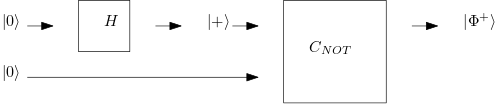
\includegraphics[width=5in]{modules/figs/m05/e09.png}
        \caption{Two-stage circuit that takes the vector $|00\rangle$ to $\left|\Phi^{+}\right\rangle$}
        \label{fig:two_stage}
    \end{figure}

\item[] \textbf{In-Class Exercise 10:} \textbf{Q.} Show the steps in applying $C_{\text{NOT}}$ to each of: $|-,+\rangle,|+,-\rangle,|-,-\rangle$. \textbf{A.}
\begin{align*}
    C_{NOT}|-,+\rangle  & = (|0\rangle\langle0| \otimes I + |1\rangle\langle1| \otimes X) (|-\rangle \otimes |+\rangle)\\
                        & = (|0\rangle\langle0||-\rangle \otimes I |+\rangle + |1\rangle\langle1| |-\rangle \otimes X |+\rangle\\
                        & = \frac{1}{\sqrt{2}}|0\rangle \otimes |+\rangle - \frac{1}{\sqrt{2}} |1\rangle \otimes |+\rangle\\
                        & = \left(\frac{1}{\sqrt2}(|0\rangle-|1\rangle)\right)\otimes |+\rangle\\
                        & = |-,+\rangle \\
    C_{NOT}|+,-\rangle  & = (|0\rangle\langle0| \otimes I + |1\rangle\langle1| \otimes X) (|+\rangle \otimes |-\rangle)\\
                        & = (|0\rangle\langle0||+\rangle \otimes I |-\rangle + |1\rangle\langle1| |+\rangle \otimes X |-\rangle\\
                        & = \frac{1}{\sqrt{2}}|0\rangle \otimes |-\rangle + \frac{1}{\sqrt{2}} |1\rangle \otimes -1|-\rangle\\
                        & = \left(\frac{1}{\sqrt{2}}(|0\rangle-|1\rangle)\right) \otimes |-\rangle\\
                        & = |-,-\rangle \\
    C_{NOT}|-,-\rangle  & = (|0\rangle\langle0| \otimes I + |1\rangle\langle1| \otimes X) (|-\rangle \otimes |-\rangle)\\
                        & = (|0\rangle\langle0||-\rangle \otimes I |-\rangle + |1\rangle\langle1| |-\rangle \otimes X |-\rangle\\
                        & = \frac{1}{\sqrt{2}}|0\rangle \otimes |-\rangle + \left(-\frac{1}{\sqrt{2}} |1\rangle \otimes -1|-\rangle\right )\\
                        & = \left(\frac{1}{\sqrt{2}}(|0\ranlge + |1\rangle)\right)\otimes |-\rangle\\
                        & = |+,-\rangle
\end{align*}


\item[] \textbf{In-Class Exercise 11:}
\begin{enumerate}
    \item [1.] \textbf{Q.} Show that $(H \otimes I \otimes I) \frac{1}{\sqrt{2}}(\alpha|000\rangle+\alpha|011\rangle+\beta|110\rangle+\beta|101\rangle)=\frac{1}{2}(|00\rangle \otimes(\alpha|0\rangle+\beta|1\rangle)+|01\rangle \otimes(\beta|0\rangle+\alpha|1\rangle)+|10\rangle \otimes(\alpha|0\rangle-\beta|1\rangle)+|11\rangle \otimes(\alpha|1\rangle-\beta|0\rangle))$ Hint: see one of the solved problems. \textbf{A.}
    \begin{align*}
        & (H \otimes I\otimes I)\frac{1}{\sqrt{2}}(\alpha|000\rangle+\alpha|011\rangle+\beta|110\rangle+\beta|101\rangle)\\
        & = \frac{1}{\sqrt{2}}\left( (\alpha(H|0\rangle\otimes I|0\rangle \otimes I|0\rangle)\\
        & + (\alpha(H|0\rangle\otimes I|1\rangle \otimes  I|1\rangle)\\
        & + (\beta(H|1\rangle\otimes I|1\rangle \otimes  I|0\rangle)\\
        & + (\beta(H|1\rangle\otimes I|0\rangle \otimes  I|1\rangle) \right)\\
        & = \frac{1}{\sqrt{2}} ( (\alpha(\frac{1}{\sqrt{2}}(|0\rangle+|1\rangle) \otimes|0\rangle \otimes|0\rangle)\\
        & + (\alpha(\frac{1}{\sqrt{2}}(|0\rangle+|1\rangle) \otimes|1\rangle \otimes|1\rangle)\\
        & + (\beta(\frac{1}{\sqrt{2}}(|0\rangle-|1\rangle) \otimes|1\rangle \otimes|0\rangle)\\
        & + (\beta(\frac{1}{\sqrt{2}}(|0\rangle-|1\rangle) \otimes|0\rangle \otimes|1\rangle )\\
        & = \frac{1}{2} ( \alpha|000\rangle +\alpha|100\rangle\\
        & + \alpha|011\rangle + \alpha|111\rangle\\
        & + \beta|010\rangle - \beta|110\rangle\\
        & + \beta|001\rangle - \beta|101\rangle\\
        & = \frac{1}{2} ( \alpha|000\rangle + \beta|001\rangle\\
        & + \beta|010\rangle + \alpha|011\rangle\\
        & + \alpha|100\rangle - \beta|101\rangle\\
        & + \alpha|111\rangle - \beta|110\rangle\\
        & = \frac{1}{2}(|00\rangle \otimes(\alpha|0\rangle + \beta|1\rangle)\\
        & +|01\rangle \otimes(\beta|0\rangle+\alpha|1\rangle)\\
        & +|10\rangle \otimes(\alpha|0\rangle-\beta|1\rangle)\\ 
        & +|11\rangle \otimes(\alpha|1\rangle-\beta|0\rangle))
    \end{align*}
    \item [2.] \textbf{Q.} Show that $(I \otimes I \otimes Z)(|10\rangle \otimes(\alpha|0\rangle-\beta|1\rangle))=|10\rangle(\alpha|0\rangle+\beta|1\rangle)$ \textbf{A.}
    \begin{align*}
        & (I \otimes I \otimes Z)(|10\rangle \otimes(\alpha|0\rangle-\beta|1\rangle))\\
        & = I |1\rangle \otimes I |0\rangle \otimes Z(\alpha|0\rangle-\beta|1\rangle) \\
        & = |10\rangle(\alpha|0\rangle+\beta|1\rangle)
    \end{align*}
\end{enumerate}

\end{enumerate}
\end{document}